% LaTeX Template for short student reports.
% Citations should be in bibtex format and go in references.bib
\documentclass[a4paper, 11pt]{article}
\usepackage[top=3cm, bottom=3cm, left = 2cm, right = 2cm]{geometry} 
\geometry{a4paper} 
\usepackage[utf8]{inputenc}
\usepackage{textcomp}
\usepackage{graphicx} 
\usepackage{amsmath,amssymb}  
\usepackage{bm}  
\usepackage[pdftex,bookmarks,colorlinks,breaklinks]{hyperref}  
%\hypersetup{linkcolor=black,citecolor=black,filecolor=black,urlcolor=black} % black links, for printed output
\usepackage{memhfixc} 
\usepackage{pdfsync}  
\usepackage{fancyhdr}
\pagestyle{fancy}



\title{Numerisk øving 1 - TFY4165}
\author{Jacob Oliver Bruun og Sondre Klyve}
%\date{}

\begin{document}
\maketitle
Denne filen inneholder resultatene fra koden. Vi tenkte det var litt greiere å presentere de tre plottene samlet i ett dokument, slik at vi også får diskutert de. Tilsvarende plott vil genereres ved å kjøre koden i main.py, men de blir så klart ikke helt like på grunn av tilfeldighetene i oppgaven.

Plottene fungerer som følger: den oransje streken viser antall lopper på hund A, og hvordan loppebestanden på hund A utvikler seg over tid. Den blå linjen viser analytisk utvikling over tid, fra formelen
\begin{equation}
  N_A(t) = \frac{N}{2}\left(1+e^{-2ct}\right)
\end{equation}
med $c= \frac{1}{N}$. Ved $\Delta t=1$ er dette et rimelig valg. Grunnen til dette er at $c$ styrer hvor fort $N_A$ stabiliserer seg mot $N$, og det gir mening at dette er omvendt proporsjonalt med antall lopper. Dersom en hund har veldig mange lopper, og det bare kan hoppe en i sekundet, vil det ta ganske lang tid før loppebestanden mellom de to hundene er lik. 
\section*{Lite antall lopper}
Vi valgte $N=6$ for lite antall lopper. Her ser vi at det blir lite mønster i plottet, nettopp fordi det er så få lopper. Dersom en loppe hopper fra den ene hunden til den andre, vil det gjøre et ganske stort utslag i antall lopper på hund A, som er reflektert i plottet.
\[
  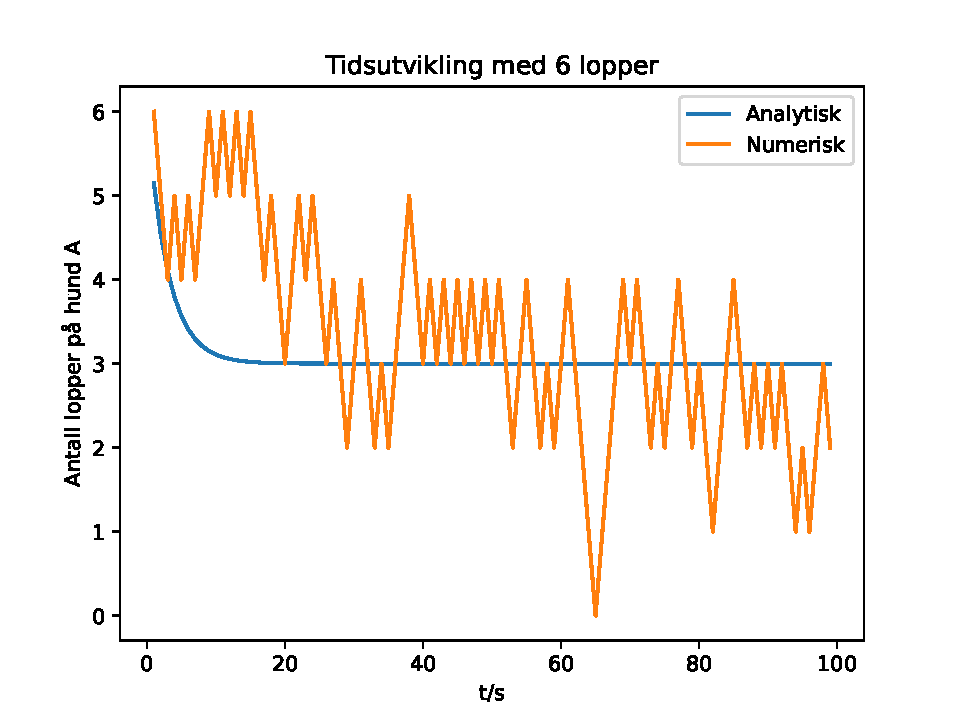
\includegraphics[scale=0.7]{figures/6_lopper.pdf}
\]
\section*{Middels stort antall lopper}
Ved $N=1000$ får vi en mer tydelig trend. Merk også at vi har brukt flere tidssteg her enn ved $N=6$. Årsaken er rett og slett at det tar lenger tid før loppefordelingen stabiliserer seg, i tråd med valg av $c$.  
\[
  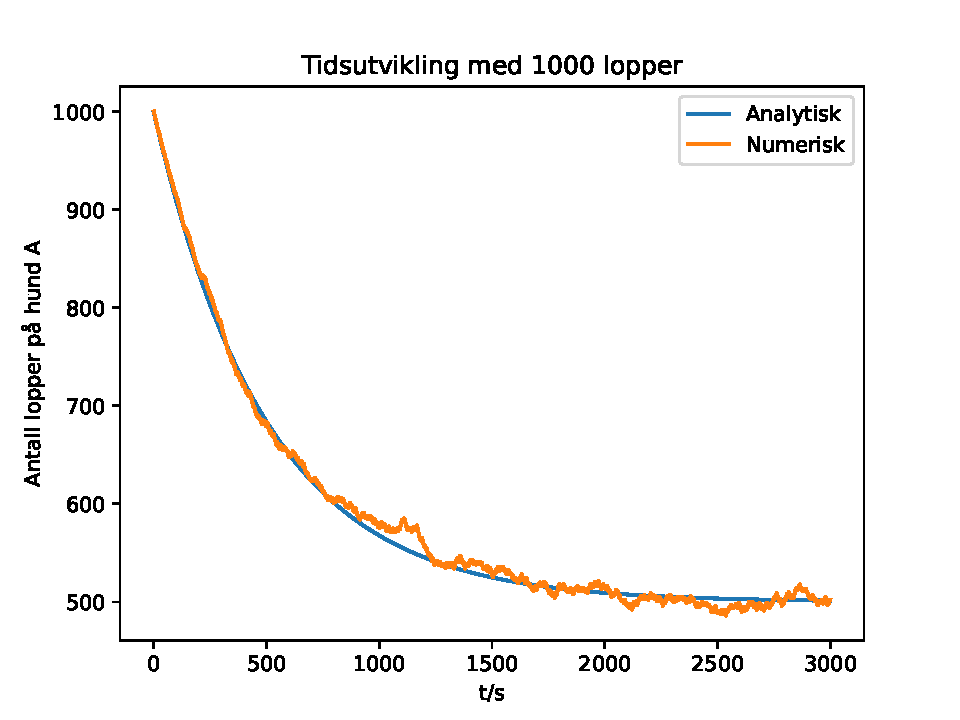
\includegraphics[scale=0.7]{figures/1000_lopper.pdf}
\]
\section*{Stort antall lopper}
Til slutt testet vi å bruke $N=20000$ lopper. Igjen har vi økt antall tidssteg, og ser at den tilfeldig genererte loppebestanden ligger veldig nært den teoretiske. 
\[
  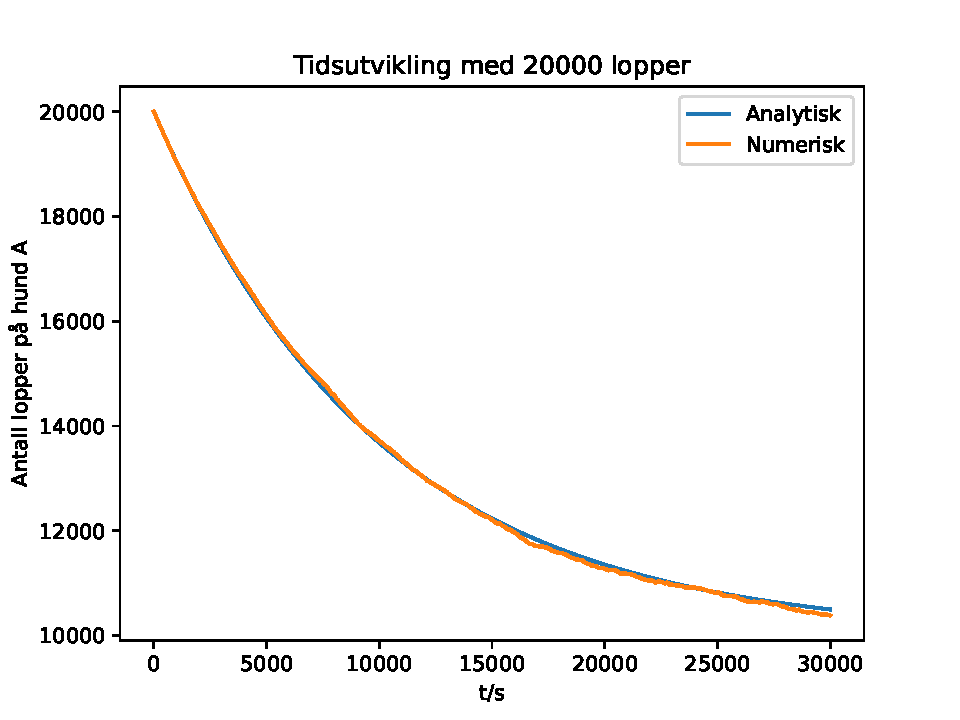
\includegraphics[scale=0.7]{figures/20000_lopper.pdf}
\]
\end{document}